\chapter{Benchmarks} 

% Benchmarks to Add (even if just the reference):

% Edge shortfall case: AUG
% Edge shortfall case: DIII-D
% Casson MAST cases
% Dickinson MAST MTM case (EPS 2013)
% Henderson MAST case (EPS 2013)
% Guttenfelder / Hornsby MTM case
% Guttenfelder / Buchholz NSTX case
% Cottier QualizKiz cases
% Self-Benchmarks for the flux tube nonspectral version:
%   Linear, RH, nonlinear
% NEMORB global benchmarks


In this section we describe a set of benchmarks. 
The benchmark cases have been chosen to maximise the effect of each of the different implemented 
terms as much as possible.
Together they give evidence for the correct implementation of the entire model. 
Linear benchmarks have been made against the GS2 code which is well established. 
Indeed the model equations are equivalent, with the exception that GKW includes the effect of a 
rigid body toroidal rotation, while GS2 does not. The implementation is to some extent similar;
both 
use a spectral approach for the plane perpendicular to the magnetic field, and finite differences for 
the other directions. 
The main difference lies in the velocity space discretisation where GKW uses $(v_\parallel, \mu)$
coordinates, whereas GS2 uses pitch angle and energy.  The GS2 velocity grid allows an efficient
implicit time integrator, while the default grid of GKW is suitable for an explicit time integrator
which facilitates parallelisation.  Also the finite difference scheme used
for GKW in the benchmarks is fourth order while GS2 has a second order scheme. 
In this section all quantities have been converted to use gyro-Bohm units. 

\section{Linear Benchmarks\label{linearbenchmarks}} 

The standard benchmark for linear problems is the growth rate of the Ion Temperature Gradient 
mode (ITG) as a function of the poloidal wave vector $k_\theta \rho_s$ for the so-called 
Cyclone base case \cite{DIM00} ($q = 1.4$, $\hat s = 0.78$, $\epsilon = 0.19$, $R / L_T = 6.9$, 
$R/L_n = 2.2$, $T_e / T_i = 1$, electro-static (zero $A_\parallel$), and adiabatic electrons). 
The growth rate for this case is shown in the right panel of Fig.~\ref{fig:cyclone-linear} as a function 
of $k_\theta\rho_s$ for various values of the normalised ion temperature gradient ($R/L_T = 6.9$,
8.28 10.35, 12.44, and 15.18) calculated with both GKW and GS2. 
As can be seen from the figure, good agreement is obtained. 
The left panel, furthermore, shows the comparison of the potential as a function of the coordinate 
along the field line ($s$) for both codes. 

\begin{figure}[htb] 
\begin{center}
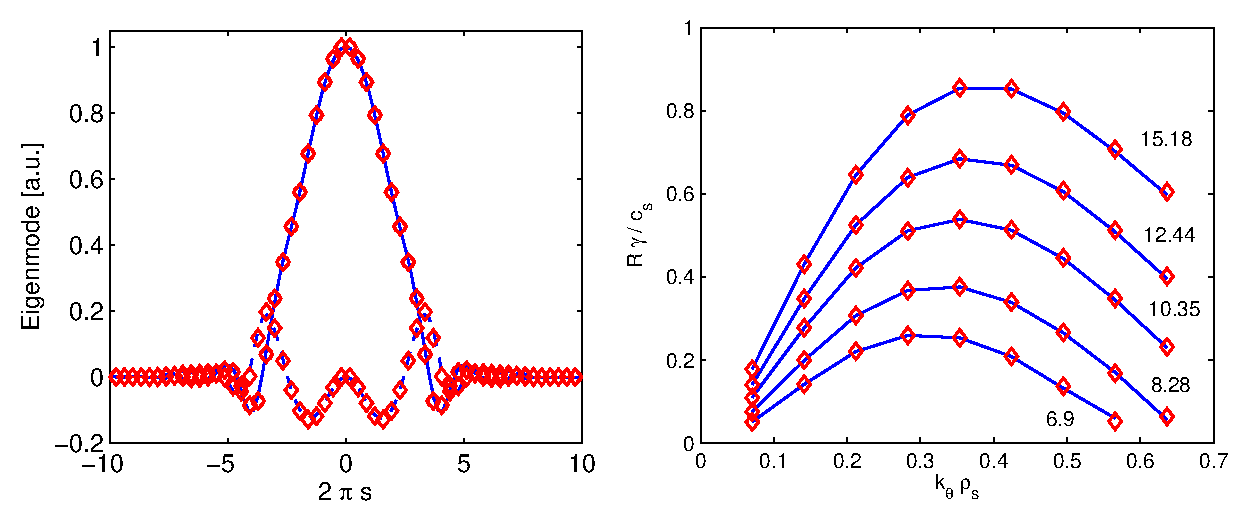
\includegraphics[width=14truecm]{cyclone-base-linear3.eps}
\caption{Left: mode structure of the Cyclone base case. The full line is the 
real part and the dotted line is the imaginary part of the potential calculated with GS2. 
The corresponding results of GKW are given by the diamonds. Right: growth rate as a function 
of $k_\theta \rho_s$ for various values of $R/L_{Ti}$ (numbers given in the figure). The full 
lines give the results of GS2 while the diamonds are the corresponding results of GKW.} 
\label{fig:cyclone-linear}
\end{center}
\end{figure}  

For nonlinear runs the proper response of the zonal flows is of utmost importance. 
The standard benchmark \cite{CAN03,JEN05,JOL07} that addresses the physics of the zonal flow / geo-acoustic 
mode is the Rosenbluth-Hinton test which was described analytically in Ref. \cite{HINROS}. 
In this benchmark the initial condition is an ion density 
perturbation with a finite (small) radial wave vector, and no dependence on either $s$ or $\zeta$.  
The adiabatic electron response is used, keeping the correction due to the flux surface average 
of the potential. The density perturbation generates a potential perturbation and excites the so
called geo-acoustic mode. This mode is damped and a small residual poloidal flow remains. Fig. 
\ref{zonalfig} gives the potential perturbation as a function of time. The relevant parameters used for this 
benchmark are $q = 1.3$, $\epsilon = 0.05$, $k_\psi \rho_s = 0.02$, electrostatic, collisionless. 
Rather large grid sizes ($N_s = 128$ and $N_{v_\parallel} = 128$) are used to avoid the recurrence 
problem \cite{CAN03}. The residual potential is given by the equation 
\begin{equation} 
{ \phi (t= \infty) \over \phi (t= 0) } = {1 \over 1 + q^2 \Theta / \epsilon^2} \qquad 
{\rm with} \qquad \Theta = 1.6 \epsilon^{3/2} + 0.5 \epsilon^2 + 0.36 \epsilon^{5/2} 
\end{equation}
The original derivation of Ref. \cite{HINROS} is accurate to lowest order in $\epsilon$ only, i.e. 
it retained only the first term $(1.6 \epsilon^{3/2})$ in $\Theta$. 
The higher order terms have been calculated in Ref.~\cite{XIA06}. 
For the parameters of the simulation shown in the left panel the residue is $\phi(t = \infty) / \phi(t= 0) 
= 0.0713$ smaller than the result of Ref. \cite{HINROS} (0.0764) but in very good agreement with the 
results of Ref. \cite{XIA06} (0.0710). The right panel shows the residue as a function of $\epsilon$. 
Good agreement with the analytic theory is obtained provided the finite $\epsilon$ effects are kept.  
\begin{figure}[htb] 
\begin{center}
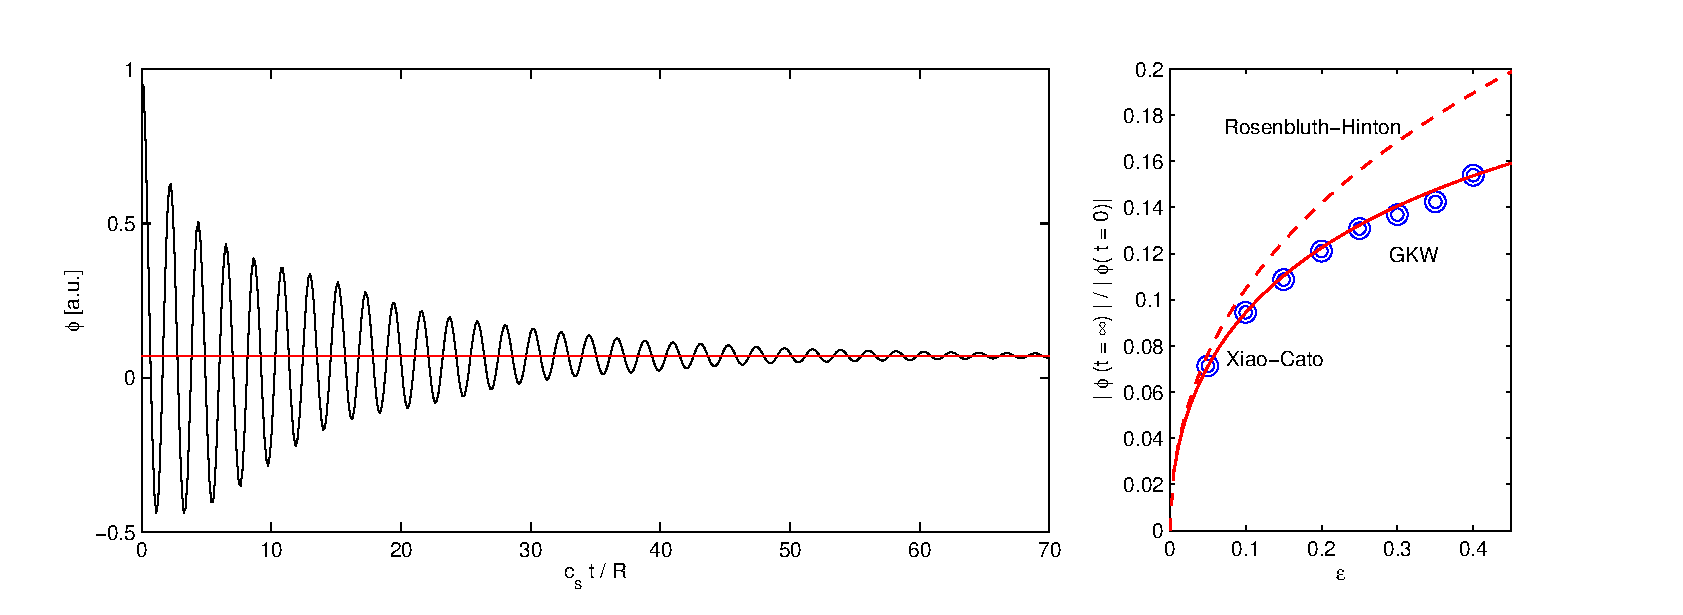
\includegraphics[width=14truecm]{RHbench.eps}
\caption{Zonal flow benchmark. Left: The potential perturbation (normalised to the potential at 
$t = 0$) as a function of normalised time, for $q = 1.3$, $\epsilon = 0.05$. The horizontal line gives the 
residual (0.0711) as predicted in Ref.~\cite{XIA06}. For this value of $\epsilon$ a numerical residual 
of 0.0713 is obtained, i.e. in agreement with the analytic result to within 0.3 \%
Right: Residual $\phi (t = \infty) / \phi(0) $ as a function of $\epsilon$ for 
$q = 1.3$. The circles are the result of GKW, the dotted line is the Rosenbluth-Hinton result \cite{HINROS} and 
the full line gives the analytic result of Xiao-Catto \cite{XIA06}. \label{zonalfig}} 
\label{overall1}
\end{center}
\end{figure}  

The Cyclone base case with adiabatic electrons does not check the correct implementation of the 
kinetic electron response, and in general is not very sensitive to the effects associated with trapped 
particles. 
The physics effects associated with kinetic electrons can be well benchmarked by considering a Trapped Electron 
Mode. A benchmark with GS2 is shown on the left of Fig.~\ref{overall2}. The parameters are 
taken from a discharge in the ASDEX Upgrade tokamak \cite{PEE05}: $\hat s = 1.07$, 
$q = 1.57$, $\epsilon = 0.177$, $T_e / T_i = 3$, $R/L_{Ti} = 0$, electro-static, collisionless, 
and with an ion to electron mass ratio of a Deuterium plasma. 
The values of the density gradient as well as the temperature gradient are scanned. 
The agreement for the growth rates is good.  

\begin{figure}[htb] 
\begin{center}
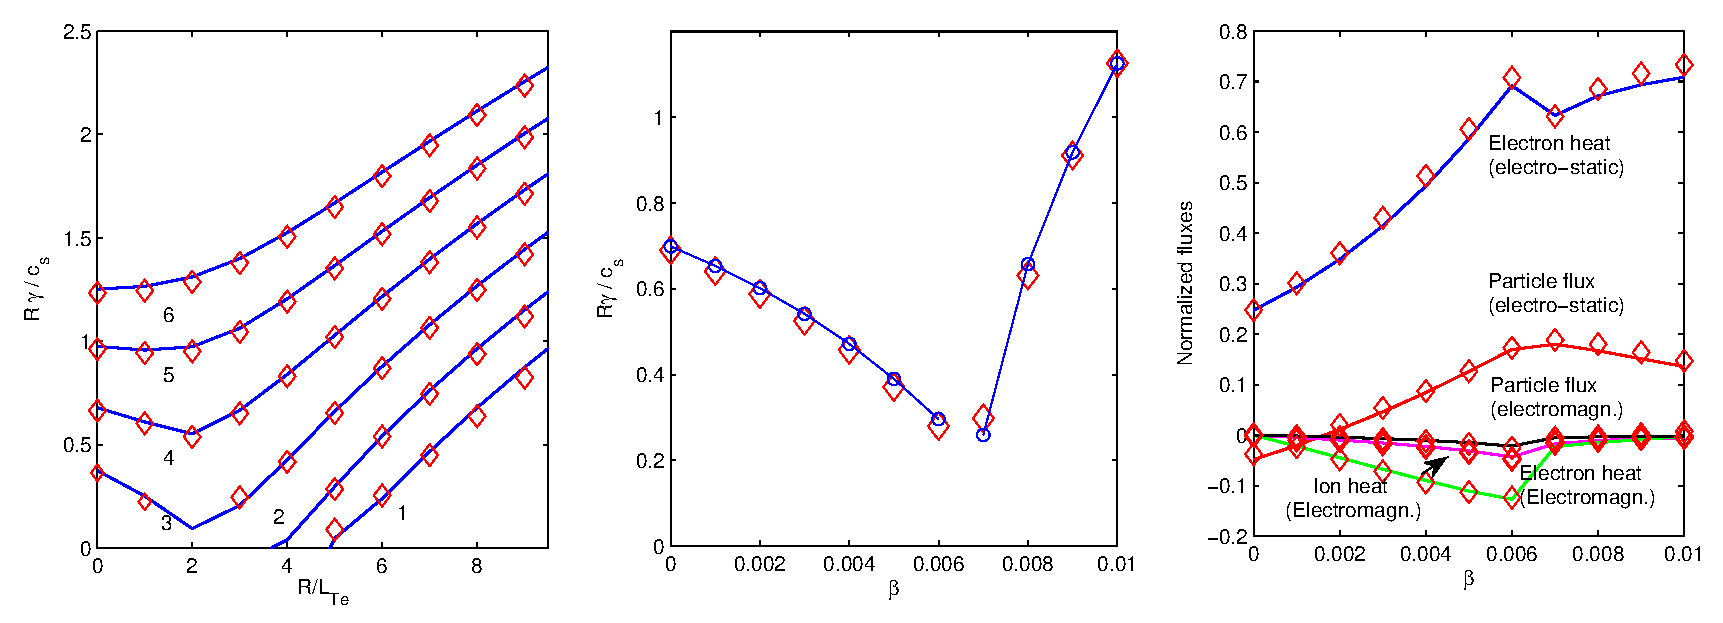
\includegraphics[width=16truecm]{overallfig-bench.eps}
\caption{Left: Benchmark of a trapped electron mode case. Shown is the normalised growth 
rate $R \gamma / c_s$ as a function of $R/L_{Te}$ for various values of $R/L_n$ indicated in 
the figure. Blue lines are the results of GS2 while red diamonds give the results of GKW. 
Middle: A benchmark of the growth rates of the ITG / Kinetic ballooning mode versus the plasma beta. 
Blue lines and circles 
are results from GS2 while red diamonds give the results of GKW. Right: The fluxes, normalised
to the ion heat flux as a function of beta. Lines give the results of GS2, while the diamonds give
the results of GKW.} 
\label{overall2}
\end{center}
\end{figure}  

Finite beta effects are tested for an ITG case increasing the plasma beta. The middle panel of 
Fig. \ref{overall2} shows the normalised growth rate as a function of the electron beta $\beta = n_e T_e 
/ (B^2 / 2 \mu_0)$ for the Waltz standard case $R/L_{Ti} = R/ L_{Te} = 9$, $R/ L_n = 3$, $q = 2$
$\hat s = 1$, $\epsilon = 0.166$ $T_e/T_i = 1$, and with a mass ratio of a Deuterium plasma. The ITG is 
stabilised by the finite beta effects and, at sufficient high values of beta, a kinetic ballooning 
mode is destabilised. The agreement for the growth rate between GKW and GS2 is again good. 
The electro-magnetic case also provides for a good benchmark of the calculation of the fluxes, since 
all fluxes (also the ones due to the magnetic flutter) are nonzero in this case. The right panel of 
Fig.~\ref{overall2} shows the comparison of the fluxes calculated by GS2 and GKW. Since for 
a linear problem the amplitude of the mode and, therefore, the magnitude of the fluxes is arbitrary, 
all fluxes have been normalised to the ion heat flux. This allows for a straightforward comparison 
between the codes. All calculated fluxes are again in good agreement. 

Effects of magnetic field compression are also tested with the linear Waltz standard test case $R/L_{Ti} = R/ L_{Te} = 9$, $R/ L_n = 3$, $q = 2$, $\hat s = 1$, $\epsilon = 0.166$, $T_e/T_i = 1$, the mode with the fastest electrostatic growth rate has been used: $k_{\perp} \rho_s = 0.3$. Fig. \ref{bpar-bm} shows that the ITG mode is hardly affected by the perturbation $B_{1 \parallel}$ but the kinetic ballooning mode is further destabilised with increasing $\beta$. Both with the growth rates and the parallel structure a good agreement with GS2 has been obtained.

\begin{figure}[htb] 
\begin{center}
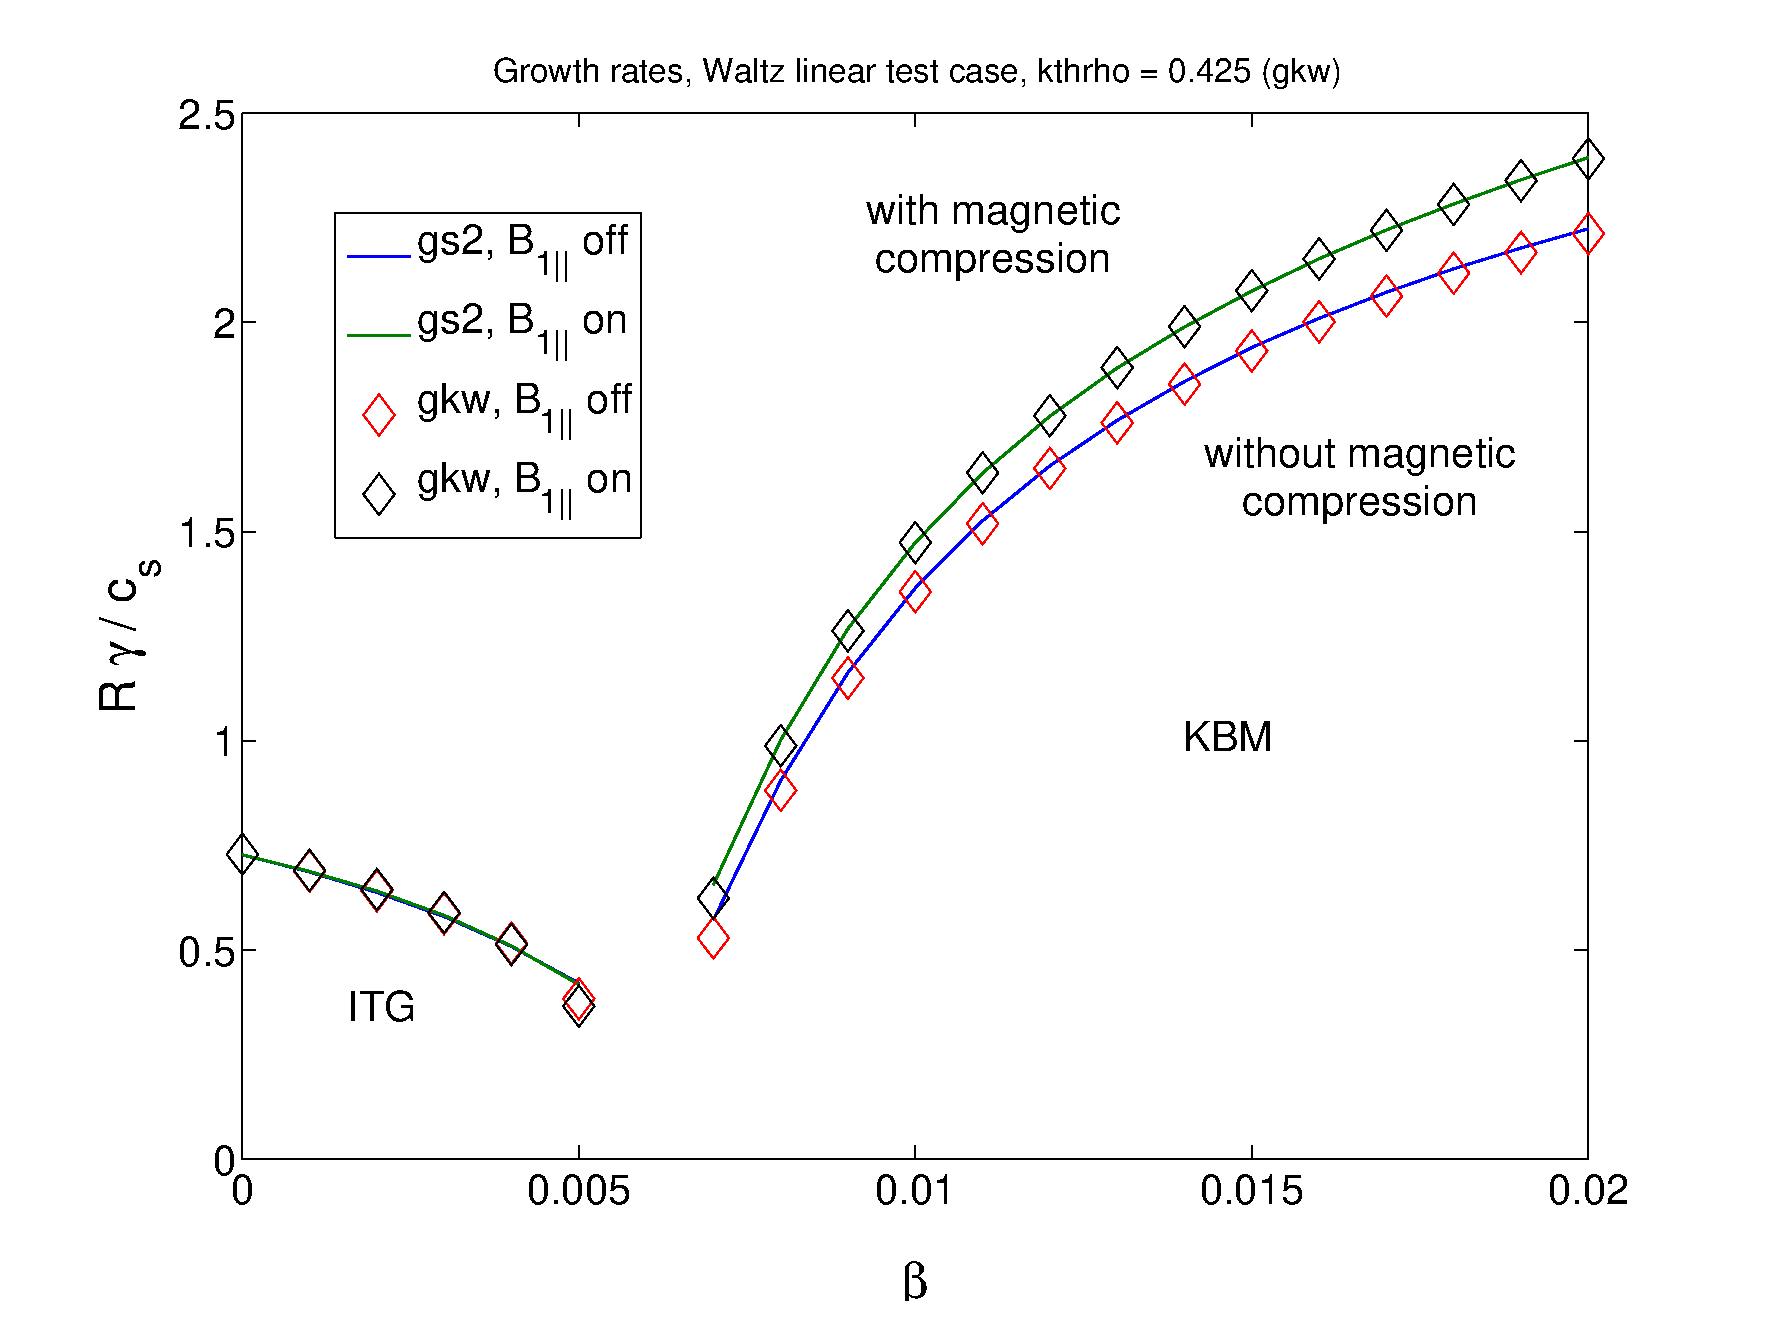
\includegraphics[scale=0.25]{bpar-growthrates-waltz-linear.eps}
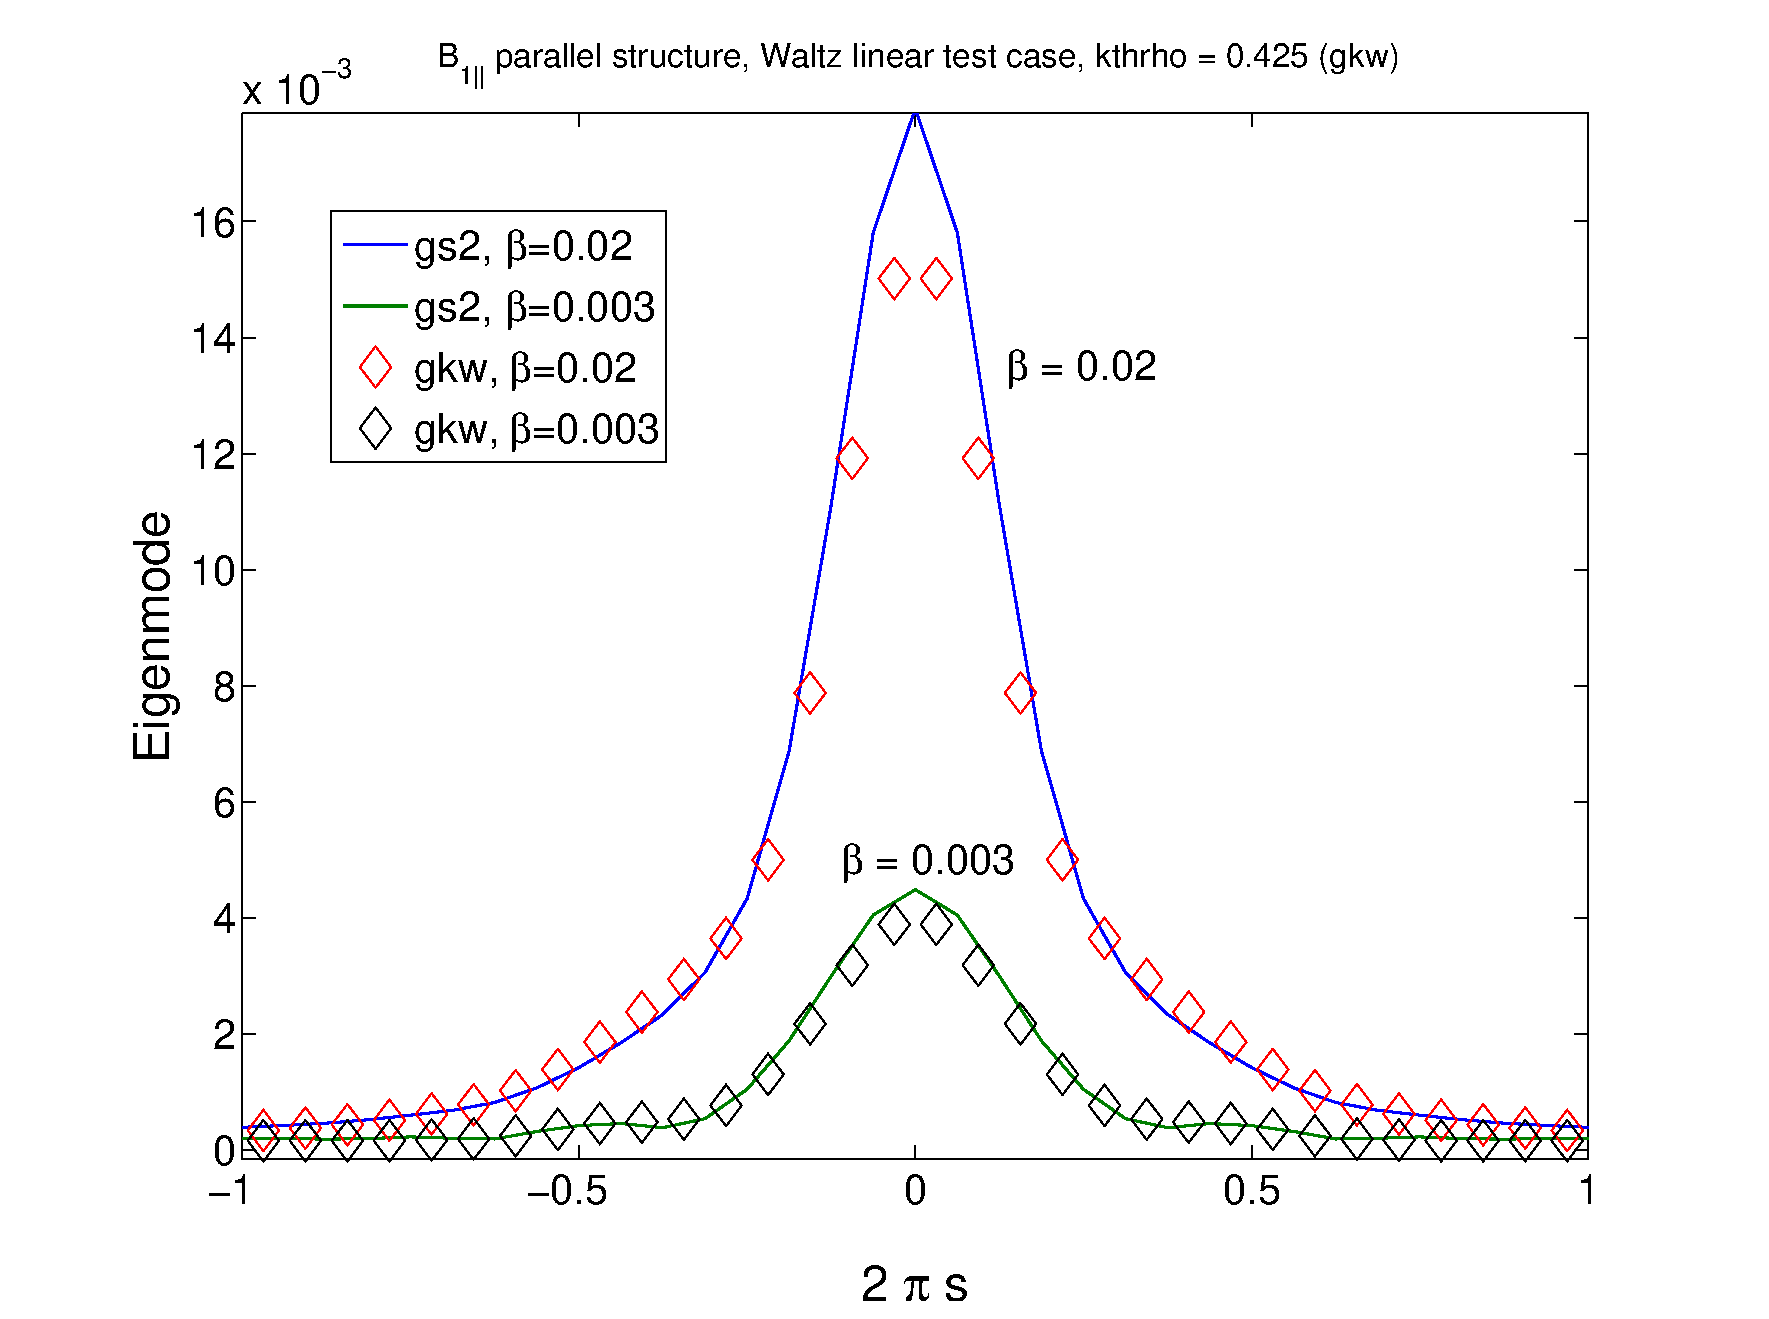
\includegraphics[scale=0.25]{bpar-parallelstructure-waltz-linear.eps}
\caption{Waltz linear test case. Left: Benchmark of growth rates of ITG and kinetic ballooning modes with magnetic field compression on and off. Right: Parallel structure of $B_{1 \parallel}$ in ITG and KBM regimes.} 
\label{bpar-bm}
\end{center}
\end{figure}

A collisionality benchmark of the pitch angle scattering against GS2 for a TEM is presented in Fig.~\ref{colls-tem}.  
To isolate the effect of e-e collisions and e-i collisions, the collisions input
variable $Z_{\rm eff}$
(a multiplier for the e-i collision rate) was varied.  Scattering of ions (off either species) made no difference for this benchmark 
(turning them on / off did not change the result of either code). This result was obtained with the Arakawa scheme and zero dissipation in $v_\parallel$. At low collisionalities, GKW convergence for a TEM requires many $v_\parallel$ points (the 64 used for this benchmark are not quite sufficient). 

\begin{figure}[htb] 
\begin{center}
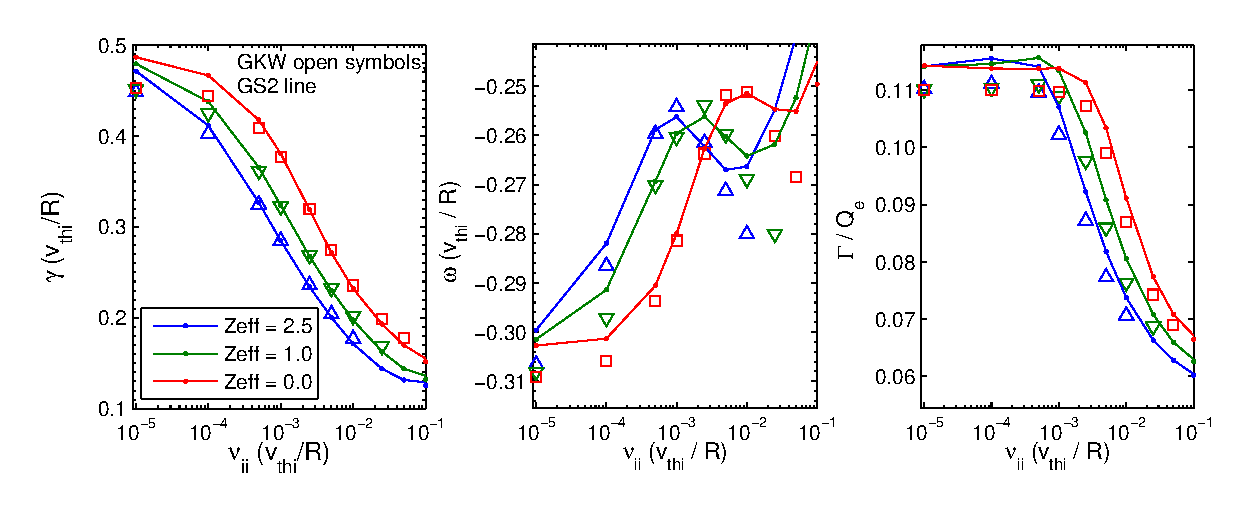
\includegraphics[scale=0.8]{bench-ee-sa-all.eps}
\caption{Collisions benchmark (pitch angle scattering) for a TEM with varying
$Z_{\rm eff}$} 
\label{colls-tem}
\end{center}
\end{figure}

The pitch angle collisions have also been benchmarked against GS2 in Ref.~\cite{PEE09scmode}, with good agreement 
obtained for the particle flux as a function of collisionality. 
The treatment of arbitrary toroidal geometry has been benchmarked against GS2 by performing an elongation scan. The parameters considered are $R/L_{Ti} = R/ L_{Te} = 8.9$, $R/ L_n = 2.85$, $q = 1.42$ $\hat s = 1.25$, $\epsilon = 0.182$, $T_e/T_i =1$ for deuterium ions and adiabatic electrons. 
The elongation of the last closed flux surface is varied from $\kappa=1.2$ to $\kappa=1.6$ and the corresponding MHD equilibrium is calculated using the CHEASE code \cite{LUT96}.
This equilibrium is then used for the calculation of the metric tensors both in GKW and GS2. 
The results for the linear growth rate as a function of $k_\theta\rho_s$ are shown in Fig.~\ref{geom-bench} showing a good agreement between the two codes.  The wavevector
normalisation (projection) in the two codes in general differs (GKW uses
$g^{\zeta\zeta}(LFS)$ while GS2 uses ${\cal E}^{\psi\zeta}$ \cite{dorland-note} which are only equivalent in `$s-\alpha$' geometry) and must
be corrected for (in this case the GKW $k_\theta$ inputs were rescaled). 
Note that the results are significantly different from the ones obtained with the simplified `$s-\alpha$' equilibrium shown by 
the dashed line (obtained with GKW).
\begin{figure}[htb] 
\begin{center}
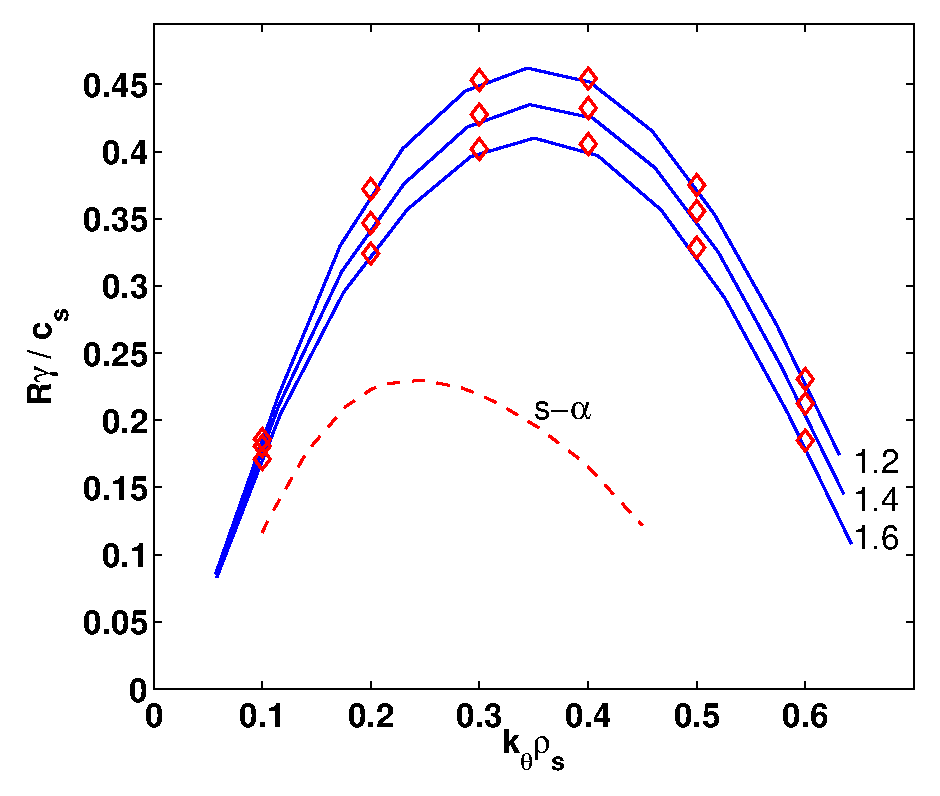
\includegraphics[width=6truecm]{geom-bench.eps}
\caption{Benchmark of the geometry treatment. The normalised growth 
rate $R \gamma / c_s$ is shown as a function of GS2 $k_\theta\rho_s$ for various values of the last closed flux surface elongation $\kappa$ indicated in 
the figure. Blue lines are the results of GS2 while red diamonds give the results of GKW. The results
obtained for the simplified `$s-\alpha$' equilibrium
with GKW are indicated by the red dashed line.} 
\label{geom-bench}
\end{center}
\end{figure}  

The effects of impurities have been benchmarked against GS2 using again the Waltz standard test case with
`$s-\alpha$' geometry $R/L_{Ti} = R/ L_{Te} = 9$, $R/ L_n = 3$, $q = 2$, $\hat s = 1$, $\epsilon = 0.166$, $T_e/T_i = 1$. Collisions were not included in this test. The left panel of Fig. \ref{impurities} shows the ITG-TEM part of the linear electro-static growth rate spectra for 4 different lithium impurity concentration. The increasing impurity density was balanced by lowering the amount of deuterium in order the preserve quasi-neutrality. This means that the increasing $n_{Li}$ leads to larger values of $Z_{\mathrm{eff}}$ which is accountable for the stabilisation of the TEM modes. 

On the middle panel of Fig. \ref{impurities} the effect of varying the type of the impurity species can be seen. The impurity density is kept at a constant 1\% in this test. Fully ionized lithium, carbon and neon and partially ionized (charge number Z=10 for both cases) iron and tungsten ions have been used. Quasi-neutrality was maintained by adjusting the deuterium density. Here, as well, the increasing $Z_{eff}$ has a stabilizing effect on the TEM modes.

And finally, the right panel of Fig. \ref{impurities} shows the effect of the two electro-magnetic perturbations, the magnetic flutter $A_{\parallel}$ and the magnetic compression $B_{\parallel}$, obtained with a lithium impurity density of 10\%. The growth rates are significantly increased compared to the electro-static cases. Apart from the longest wavelength modes a good agreement is found between the two codes. 

\begin{figure}[htb]
\begin{center}
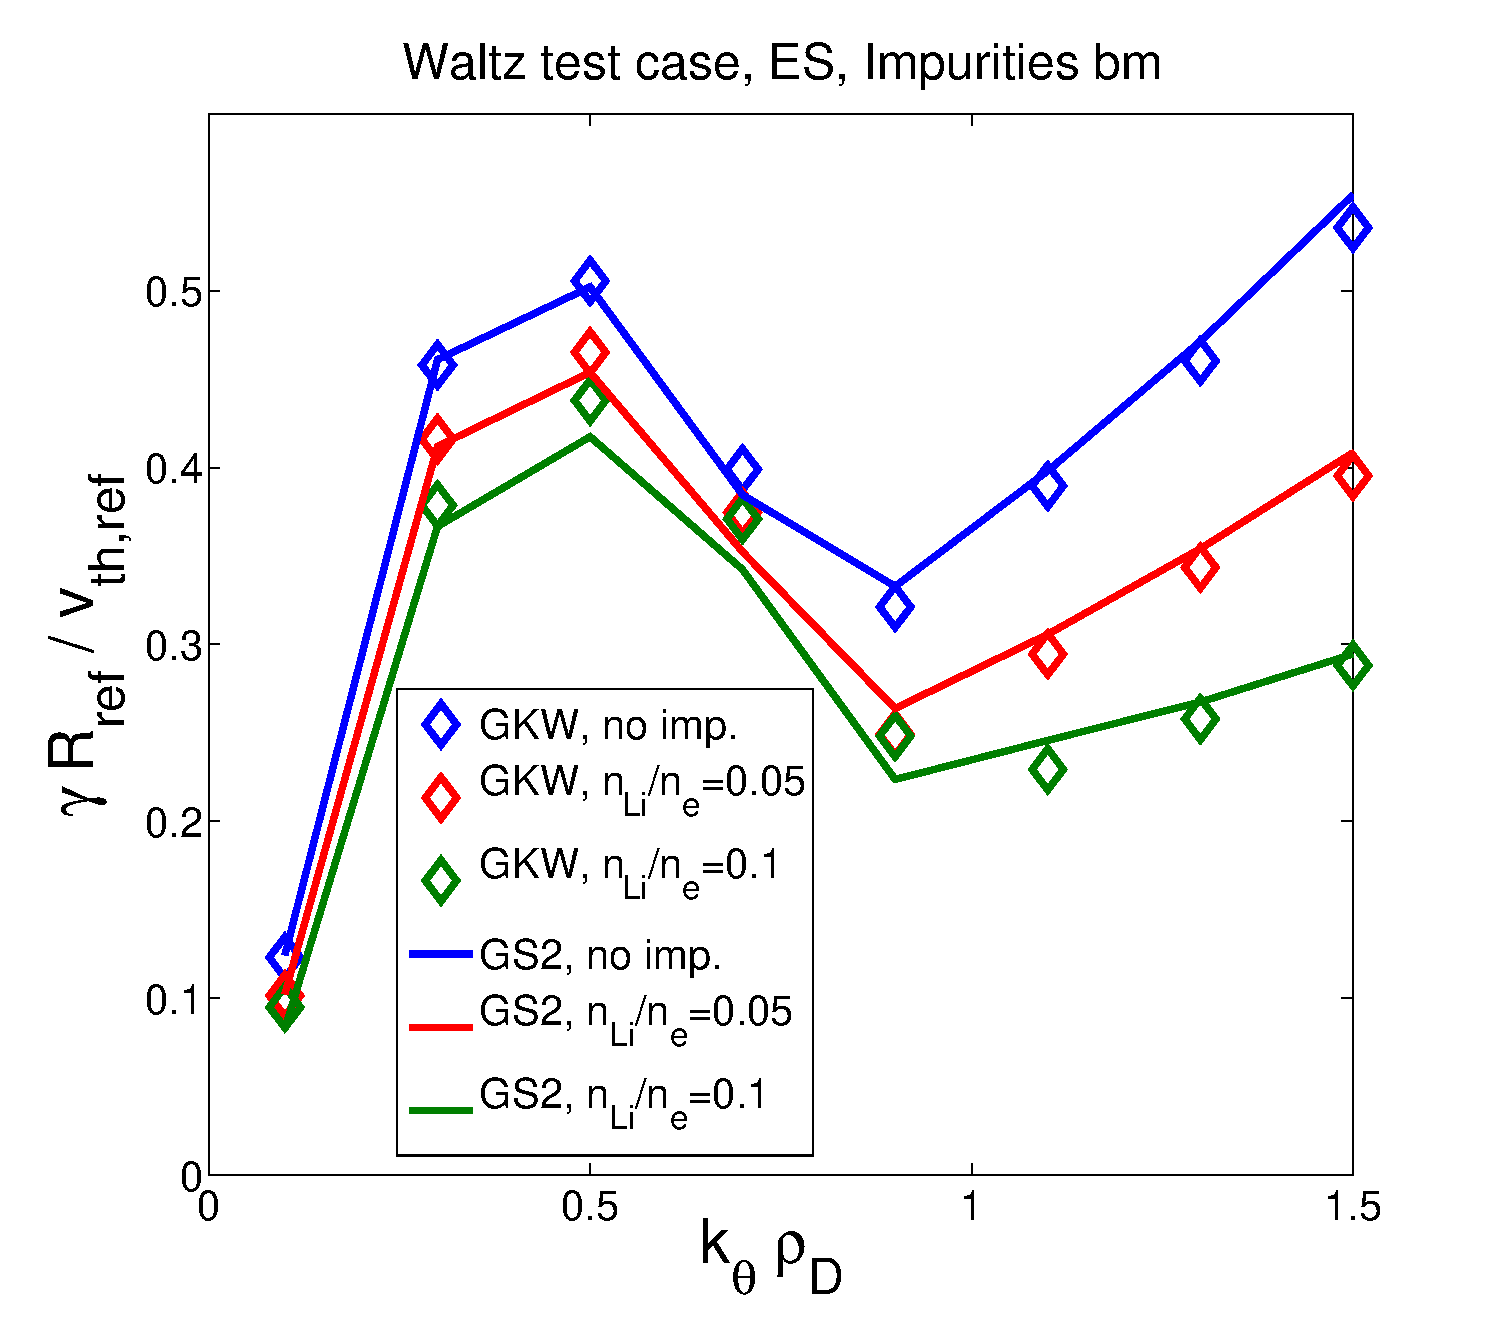
\includegraphics[scale=0.21]{waltz-gr-es-sa-nocoll.eps}
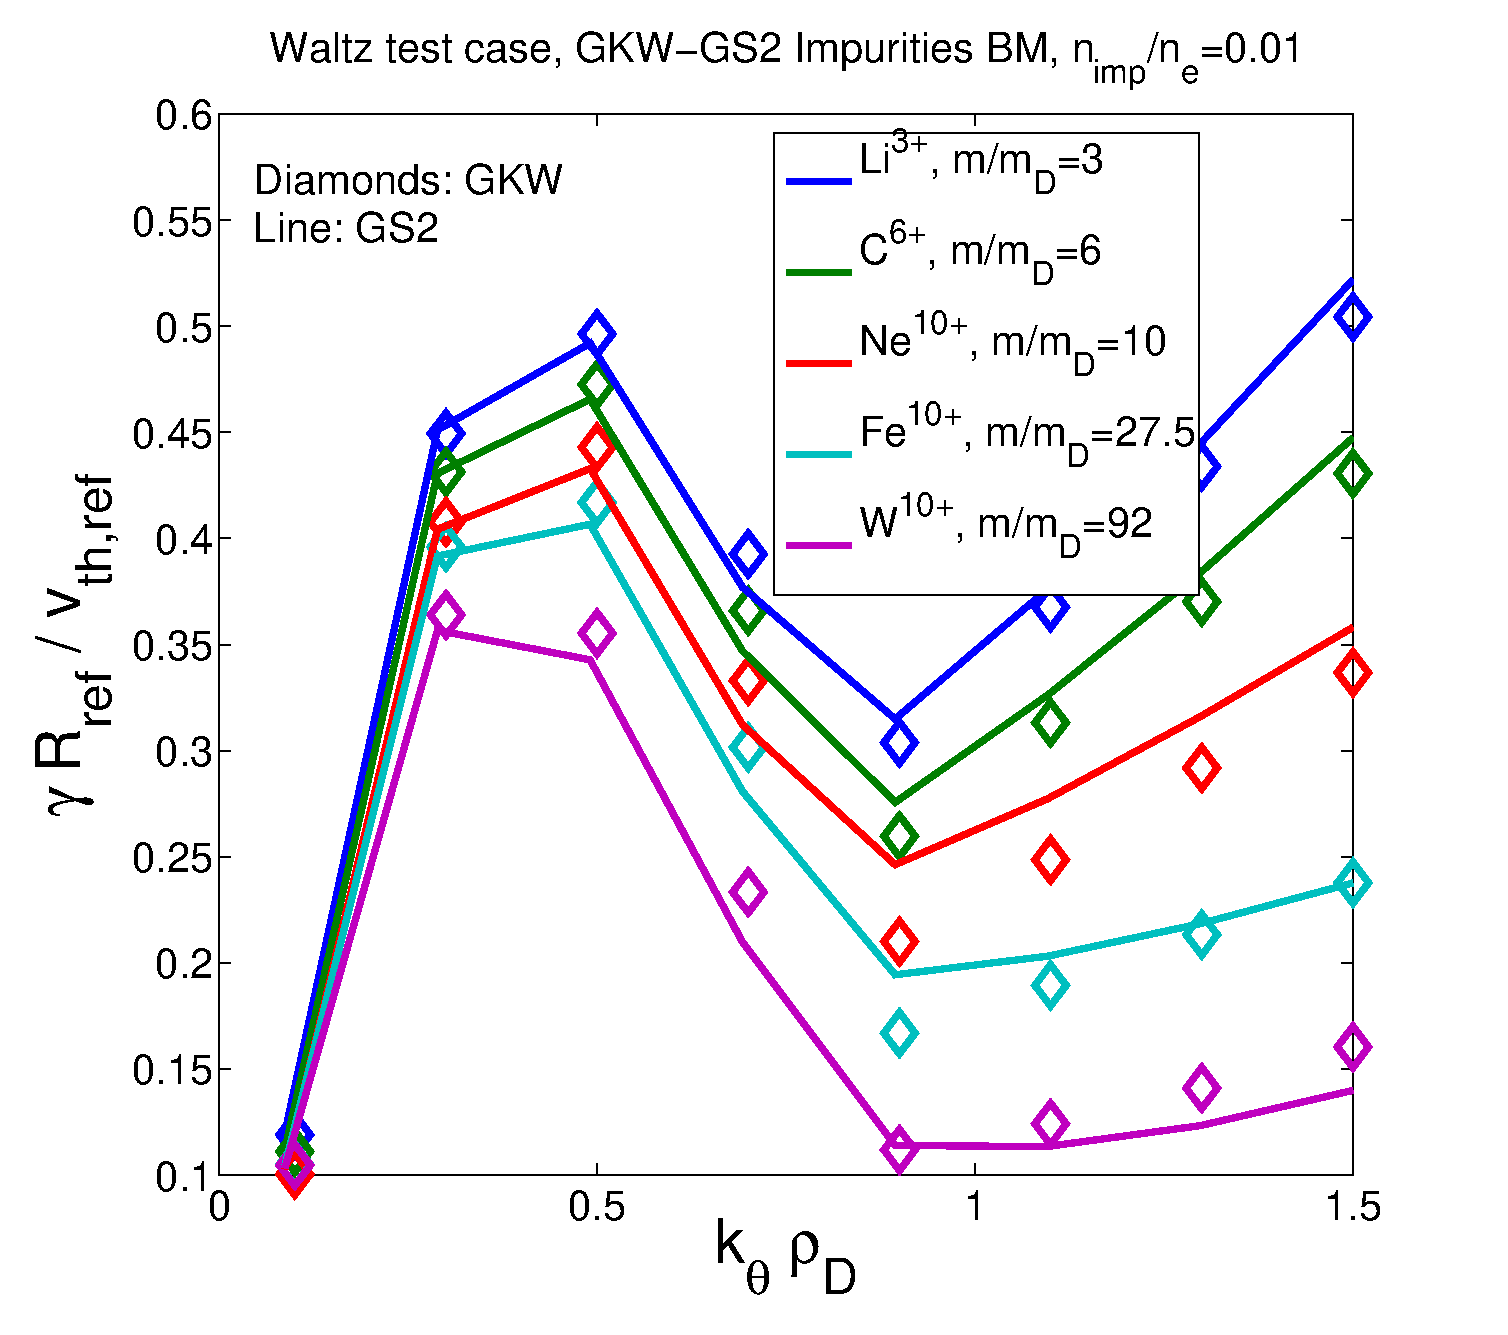
\includegraphics[scale=0.21]{waltz-gr-es-sa-Zimp-nocoll.eps}
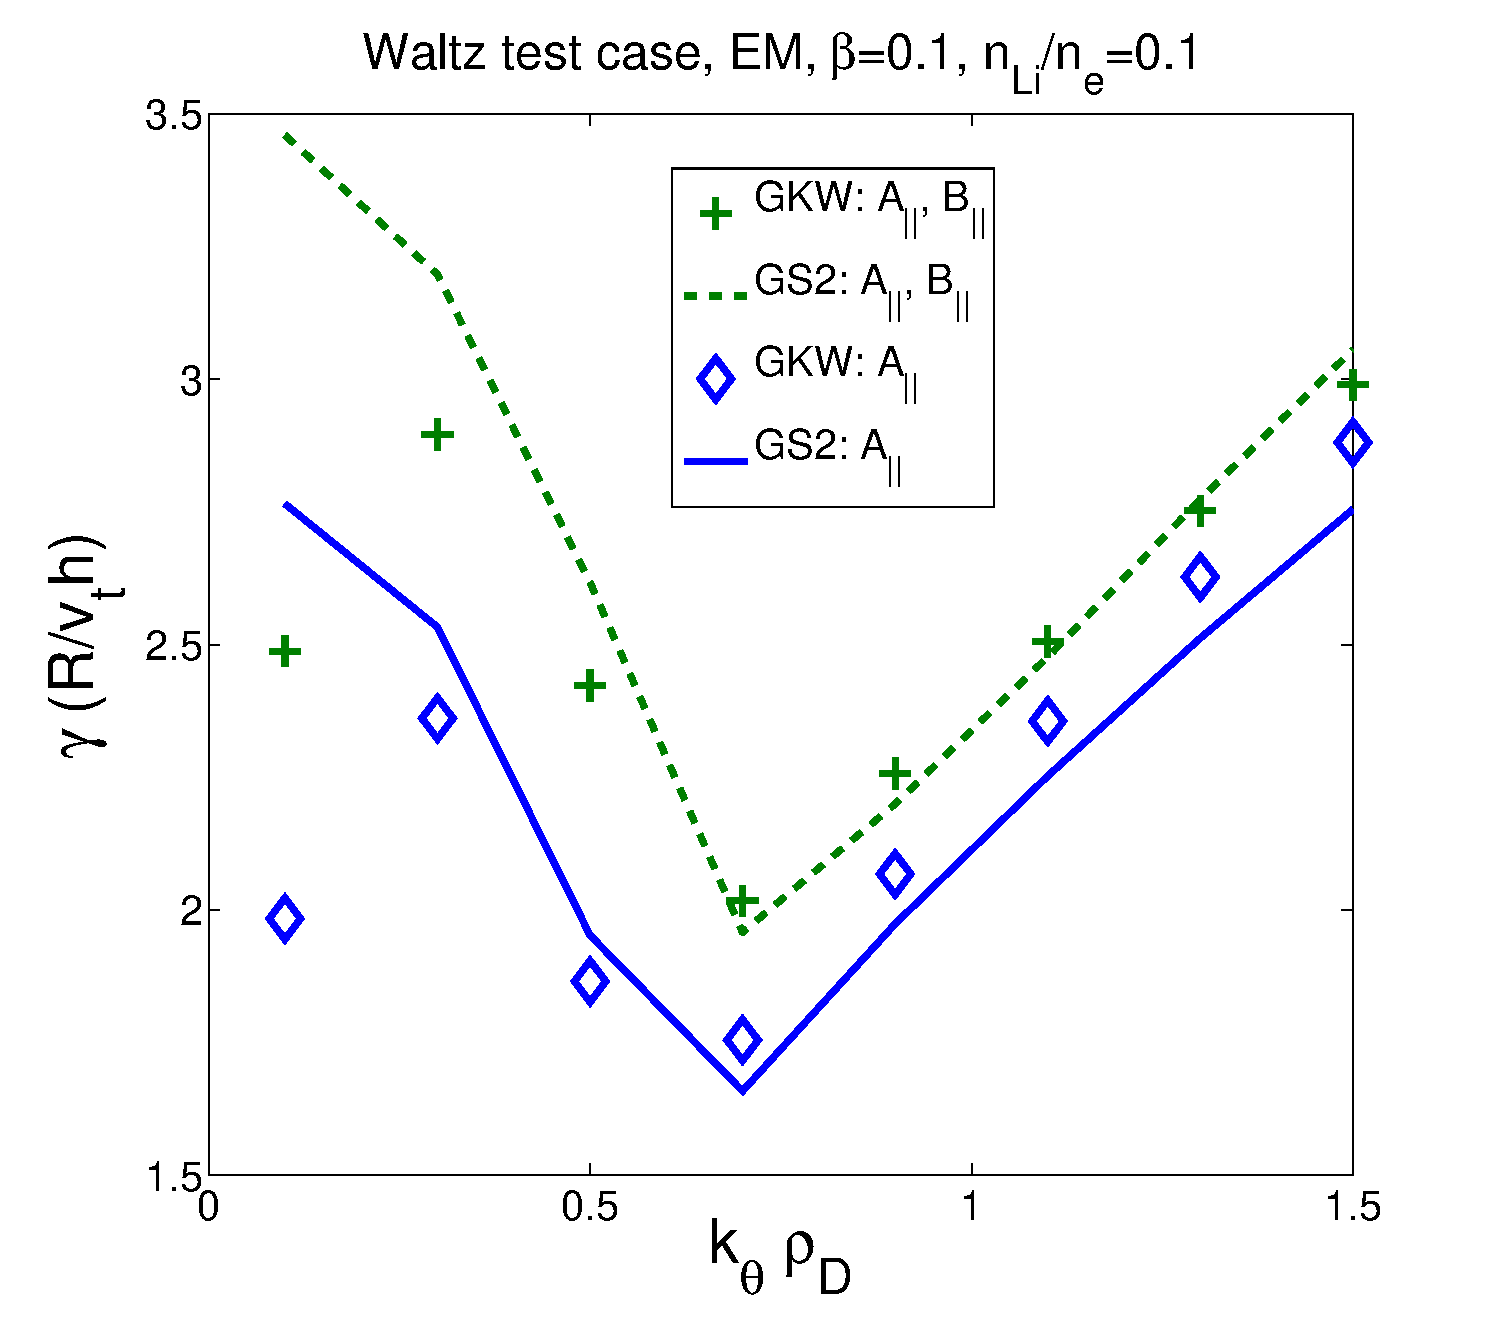
\includegraphics[scale=0.21]{waltz-gr-em-sa-nocoll.eps}
\caption{Benchmark of impurity treatment, growth rates of the Waltz standard test case with `$s-\alpha$' equilibrium without collisions. Line: GS2, diamonds: GKW. Left panel: effect of varying the Li impurity concentration, electro-static. Middle panel: effect of changing the impurity species, electro-static. Right panel: effect of the electro-magnetic perturations. Green line: fully electro-magnetic, both $A_{\parallel}$ (magnetic flutter) and $B_{\parallel}$ (magnetic compression) are retained. Blue line: only $A_{\parallel}$ is included.}
\label{impurities}
\end{center}
\end{figure}

The Miller geometry has been benchmarked against GS2, also for the adiabatic Waltz Standard case, with $\epsilon$ changed to 0.266.  As for the general geometry benchmark, the
different wavevector normalisations must be corrected (in this case the GS2 $k_\theta$ inputs were rescaled), after which very good agreement is found (Fig. \ref{miller}.).  The squareness and elevation have not been
benchmarked since GS2 does not have these parameters.  Some of the Miller parameters are defined differently in the two codes and require a simple conversion.

\begin{figure}[htb]
\begin{center}
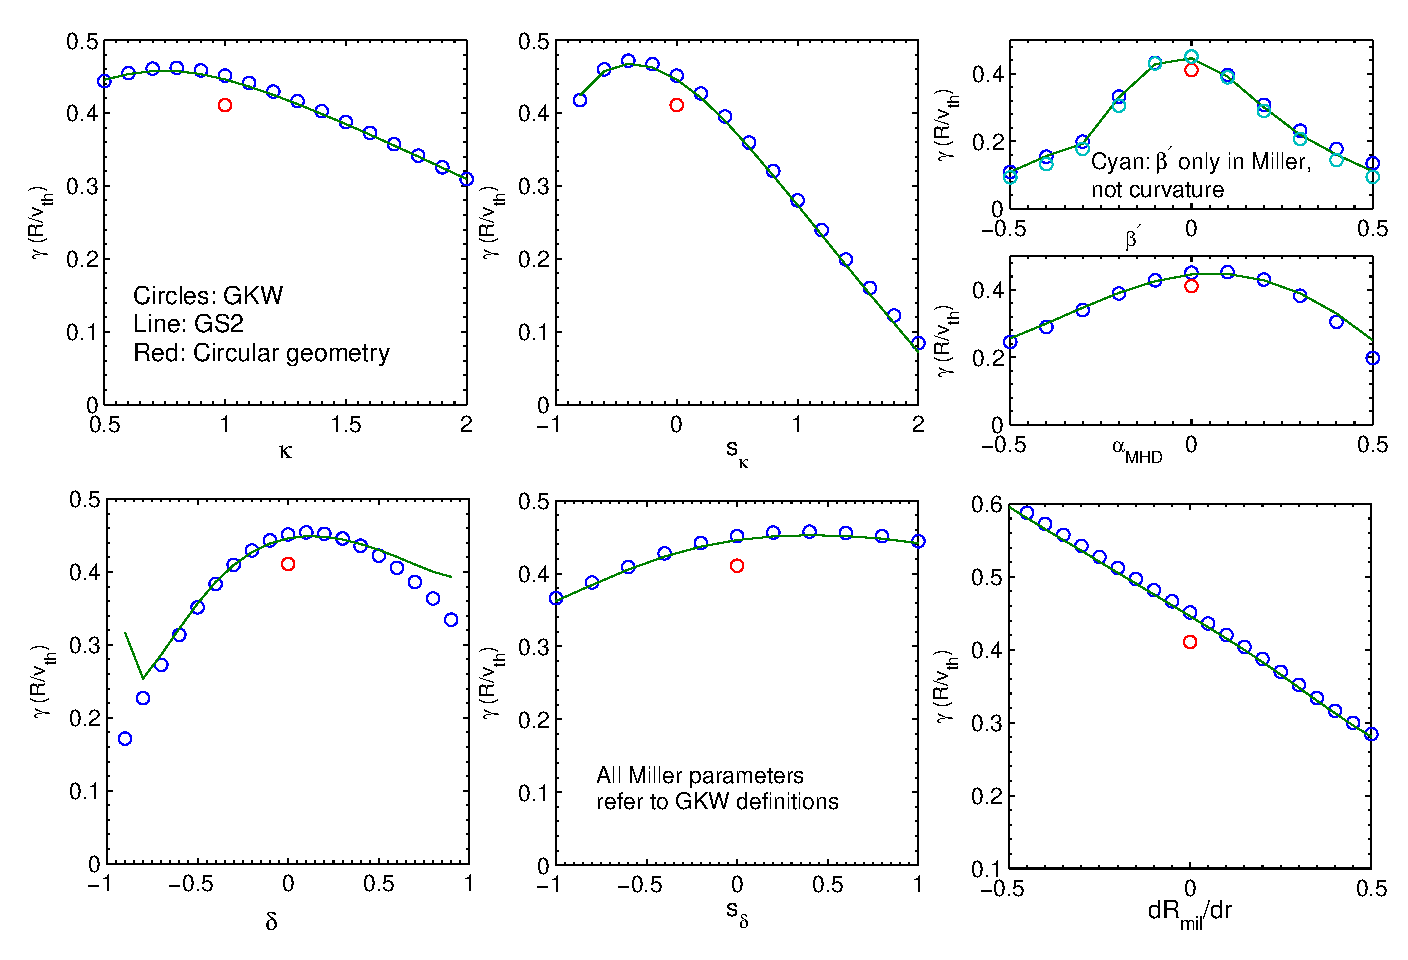
\includegraphics[scale=0.65]{geom-miller.eps}
\caption{Benchmark of the Miller geometry for the growth rates of the adiabatic
Waltz standard case with $\epsilon=0.266$ and GKW $k_\theta \rho_i=0.43$. Line: GS2, Circles: GKW.  The Miller
parameters shown on the horizontal axes refer to the GKW definitions.}
\label{miller}
\end{center}
\end{figure}


\section{Nonlinear benchmarks} 

\begin{figure}[thb] 
\begin{center}
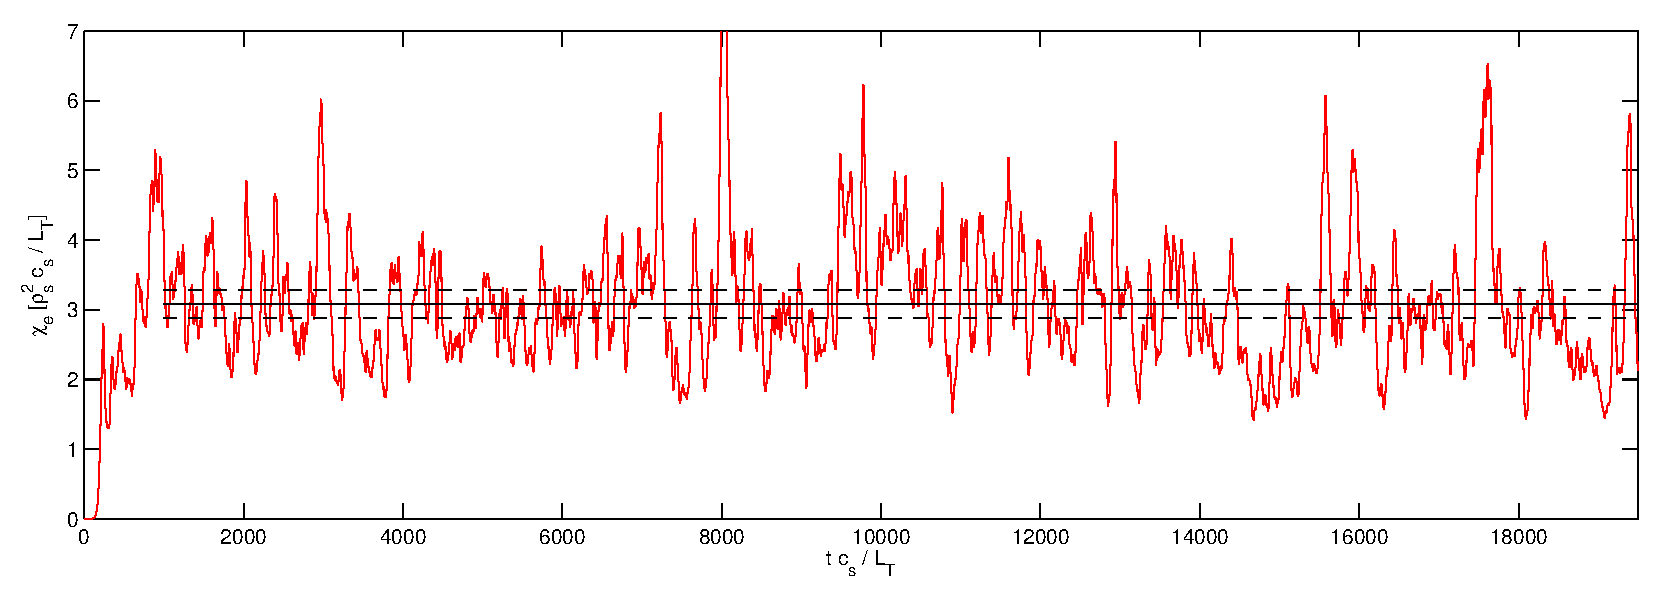
\includegraphics[width=12 truecm,clip]{heatflux.eps}
\caption{GKW results of the electron heat flux expressed as a heat conduction coefficient (normalised
to $\rho_e^2  c_e / L_T$ with $c_e = \sqrt{T_e/m_e}$) as a function of normalised time ($t_{NN} = tc_e/L_T$)
for the Nevins ETG benchmark}
\label{cyclone-nl} 
\end{center}
\end{figure} 

For the nonlinear solution there are two well established benchmark cases for which several codes have 
been compared: the cyclone base case, and the Nevins ETG benchmark. 
GKW has been benchmarked against the European gyrokinetic codes for the Cyclone case 
in Ref.~\cite{Euro-bench}. 

Here we  describe the alternative ETG benchmark of Nevins \cite{NEV08}. The 
parameters for this case are the same as those of the Cyclone base case ($R/L_T = 6.9$, 
$R/L_n = 2.2$, $q = 1.4$, $T_e / T_i = 1$, $\epsilon = 0.18$) with only the magnetic shear 
changed to $\hat s = 0.1$. For this case the electron dynamics is simulated while the 
ions are assumed adiabatic. The latter response does not include the flux surface average 
of the electro-static potential, i.e. the response is proportional to $n_i \phi / T_i$.  
To obtain the same results as published in Ref.~\cite{NEV08} we have used (and must use)
the same number of bi-normal modes $N_{\rm mod} = 8$, and mode spacing $(k_\perp \rho_s)_{\rm max} 
= 0.69$. The radial grid spacing is $\Delta (k_r \rho_s) =0.0619$ with $N_x = 41$ (both 
positive and negative wave vectors counted).  Finally, $N_\mu = 8$, $N_{v_\parallel} = 
16$, and $N_s = 16$. 

\begin{figure}[thb] 
\begin{center}
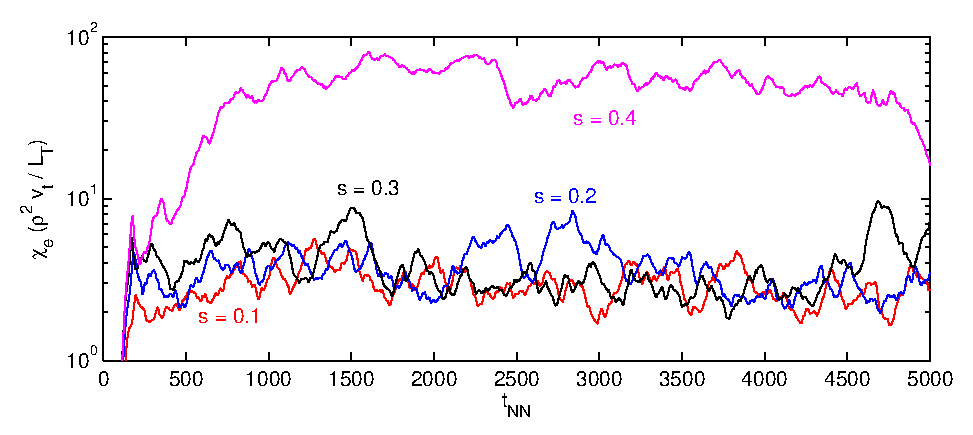
\includegraphics[width=12truecm]{shear-scan3.eps}
\caption{GKW results of the electron heat conduction coefficient for different values
of the magnetic shear}
\label{cyclone-nl2} 
\end{center}
\end{figure}  

Figure~\ref{cyclone-nl} shows the normalised electron heat flux as a function of the normalised
time. Averaging over the time interval ($1000 < t c_e / L_T < 19500$), 
GKW predicts a heat diffusion coefficient $\chi_e = 3.08 \pm 0.19$ in good agreement with the 
value $\chi_e = 2.95\pm 0.15$ reported in Ref. \cite{NEV08}. The ETG case is 
sensitive to the magnetic shear. For values $\hat s > 0.3$ no convergence is found in the simulations 
reported in Ref. \cite{NEV08}. GKW reproduces this result as shown in Fig. \ref{cyclone-nl2}.

\begin{figure}[htb] 
\begin{center}
\subfigure[Benchmark with GYRO]{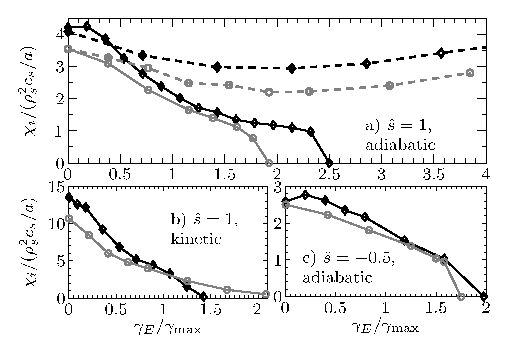
\includegraphics[height=145pt]{exb-benchmark}}
\subfigure[Benchmark with GS2]{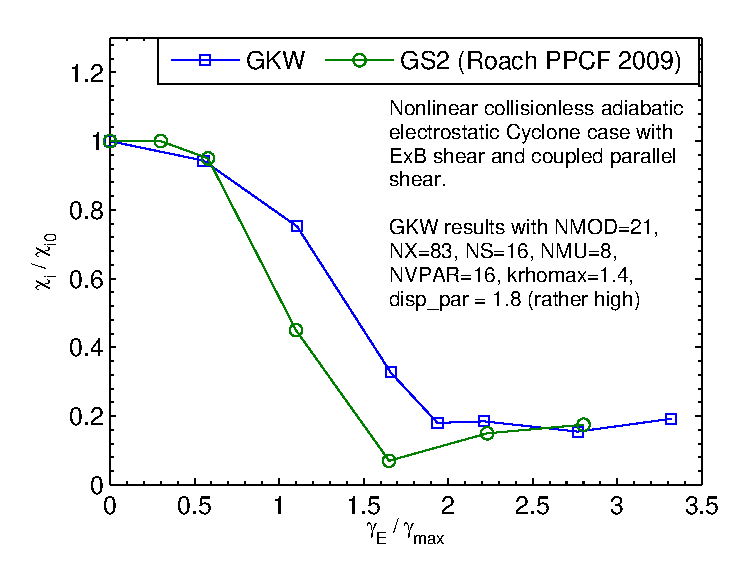
\includegraphics[height=150pt]{GKW-GS2-exb}}
\caption{Left: GKW benchmark of background ExB shearing with GYRO for Waltz standard case parameters. GKW results (diamonds) for
 adiabatic electrons, kinetic electrons, and adiabatic with $\hat s = -0.5$, are compared to the equivalent GYRO results (circles) from Tables II, III, IV and V  of Ref. \cite{KIN05}. The dashed lines include coupled
parallel velocity shear for purely toroidal rotation with $u^\prime=12\gamma_E$.  Right: GKW benchmark of background ExB shearing with GS2 results reported in Ref. \cite{ROA09} for Cyclone case parameters.  Both codes were run including coupled parallel velocity shear for purely toroidal rotation.  $\gamma_{\rm max}$ is the maximum linear growth rate at $\gamma_E=0$.}
\label{exb-gyro} 
\end{center}
\end{figure} 

The background ExB shear stabilisation 
has been successfully benchmarked against GYRO results as reported in Ref. \cite{CAS09}.  This result for the Waltz standard case 
is included again here for convenience in Fig. \ref{exb-gyro}.  GKW has also been checked against 
the GS2 results reported in Ref. \cite{ROA09} for the Cyclone case, also shown in Fig. \ref{exb-gyro}.  Both of these comparisions were against existing results, i.e. no further attempt to examine the convergence of the GYRO and GS2 results has been made.  Detailed convergence testing for the GKW results is described in Refs. \cite{Casson-Thesis} and \cite{exb-dissip}.  This study revealed that it is preferable to use some radial hyperdissipation and minimal parallel dissipation at high shear rates (see also Sec. \ref{sec.dissip}.) (not the case for these figures) which can improve the agreement at high shear rates to better than that shown in Fig. \ref{exb-gyro}.

Towards the edge, nonlinear and electromagnetic physics can be significantly more complex than
the ITG dominated Cyclone and GA-STD cases,
and benchmarking in this area is an active area of research.  
For L-mode ASDEX-Upgrade plasmas, GKW has been sucessfully benchmarked with GENE 
for four nonlinear electromagnetic cases using full geometry, and full collisions.  The results 
are reported in in Refs. \cite{FAB13} and \cite{TOL13}.  
Benchmarking for the the DIII-D `shortfall' case is in progress and 
is reported in ITPA presentations of C. Holland and Y. Camenen.

\subsection{Global Benchmarks}

Can be found in the Ringberg 2012 presentation of A.G Peeters on the GKW webpages under Talks..


\vskip 0.2 truecm

\noindent{\bf Acknowledgements} The authors want to thank W. Dorland and M. Kotschenreuther 
for making the GS2 code available, as well as A. Marinoni for his contribution to the geometry benchmark.
One of the authors (AGP) would also like to thank Bruce D. Scott for 
his tutorials and insights into the subject which he has been able to follow over many years.

% related to auctex mode and latex-preview-mode in Emacs:
%%% Local Variables:
%%% mode: latex
%%% TeX-master: "doc"
%%% End:
